\documentclass{article} % For LaTeX2e
\usepackage{nips15submit_e,times}
\usepackage{hyperref}
\usepackage{url}
\usepackage{amsmath}
\usepackage{amsfonts}
\usepackage{graphicx}
\usepackage{caption}
%\usepackage{subcaption}
\usepackage{subfig}
\usepackage{tabulary}
\usepackage{soul}
\usepackage{color}
\usepackage{xcolor}
%\usepackage{natbib}
%\usepackage[style=numeric,sorting=none,maxnames=2]{natbib}
\usepackage[square,comma,sort&compress,numbers]{natbib} 
\bibliographystyle{unsrt85}

\captionsetup{font=small}


\newcommand{\comm}[1]{}
\newcommand{\given}{\,|\,}
\newcommand{\expectation}{\mathbb{E}}
\newcommand{\kldiv}{\mathrm{D}_{\rm KL}}
\newcommand{\klBars}{\,\|\,}
\newcommand{\sigmoid}{\boldsymbol{\sigma}}
\newcommand{\hlang}{h^{lang}}
\newcommand{\hlangall}{\boldsymbol{h^{lang}}}
\newcommand{\hdec}{h^{dec}}
\newcommand{\henc}{h^{enc}}
\newcommand{\readop}{\mathit{read}}
\newcommand{\writeop}{\mathit{write}}
\newcommand{\encoder}{\mathit{LSTM}^{enc}}
\newcommand{\decoder}{\mathit{LSTM}^{dec}}
\newcommand{\canv}{c}
\newcommand{\lat}{z}
\newcommand{\Lat}{Z}
\newcommand{\numSamples}{L}
\newcommand{\sampleIdx}{l}
\newcommand{\LatSample}{\tilde{Z}}
\newcommand{\icaption}{{\bf{y}}}
\newcommand{\oimage}{{\bf{x}}}
\newcommand{\post}{q}
\newcommand{\prior}{p}
\newcommand{\loss}{\mathcal{L}}
\newcommand{\lloss}{\mathcal{L}^{z}}
\newcommand{\rloss}{\mathcal{L}^{x}}
\newcommand{\hlc}[2][yellow]{{\sethlcolor{#1}\hl{#2}}}

\definecolor{0}{RGB}{247,251,255}
\definecolor{1}{RGB}{222,235,247}
\definecolor{2}{RGB}{198,219,239}
\definecolor{3}{RGB}{158,202,225}
\definecolor{4}{RGB}{107,174,214}
\definecolor{5}{RGB}{66,146,198}

\newcommand{\hlczero}[1]{\hlc[0]{#1}}
\newcommand{\hlcone}[1]{\hlc[1]{#1}}
\newcommand{\hlctwo}[1]{\hlc[2]{#1}}
\newcommand{\hlcthree}[1]{\hlc[3]{#1}}
\newcommand{\hlcfour}[1]{\hlc[4]{#1}}
\newcommand{\hlcfive}[1]{\hlc[5]{#1}}


\newenvironment{myfont}{\fontfamily{[pcr]}\selectfont}{\par}
\DeclareTextFontCommand{\textmyfont}{\myfont}

\setlength{\abovecaptionskip}{5pt} % Chosen fairly arbitrarily
\setlength{\belowcaptionskip}{5pt} % Chosen fairly arbitrarily

\title{Generating Images From Captions\\ With Attention}

\author{
Elman Mansimov, Emilio Parisotto, Jimmy Lei Ba \& Ruslan Salakhutdinov\\
Department of Computer Science\\
University of Toronto\\
Toronto, Ontario, Canada \\
\texttt{\{emansim,eparisotto,rsalakhu\}@cs.toronto.edu}, \texttt{jimmy@psi.utoronto.ca}
}

\newcommand{\fix}{\marginpar{FIX}}
\newcommand{\new}{\marginpar{NEW}}
\graphicspath{{../}}
\begin{document}

\maketitle

\begin{abstract}
At the end.
\end{abstract} 

\section{Introduction}
Statistical natural image modelling remains a fundamental problem in computer vision and image understanding.
Despite advances in variational generative models \cite{kingma_vae}\cite{gregor_draw} and Generative Adversarial Networks (GANs) \citep{goodfellow_gan}\cite{denton_lapgan}, 
generative models of images studied previously often defined distributions that were restricted to being either unconditioned or conditioned on simple structured annotations, for example classification labels.
In real world applications, however, images rarely appear in isolation as they are often accompanied by unstructured textual descriptions, such as on web pages and in books. 
The additional information from these descriptions could be used to simplify the image modelling task. Moreover, learning generative models conditioned on text also allows a better understanding of the generalization performance of the model, as we can create textual descriptions of completely new scenes not seen at training time. 

\comm{
Significant amount of recent works has been focused on generating captions from images \citep{karpathy_captions}, \citep{xu_captions}, \citep{kiros_captions} and etc. By contrast, image understanding may also be studied by generating images correctly interpreting the text description. 
Generating high dimensional realistic images from their descriptions is a more difficult approach that combines two challenging components of language modelling and image generation.  
}

In this paper, we address the problem of image generation from unstructured natural language captions. By extending the Deep Recurrent Attention Writer (DRAW)\cite{gregor_draw}, our model iteratively draws patches on a canvas, while attending to the relevant words in the description. Overall, the main contributions of this work are the following: we introduce a conditional alignDRAW model, a generative model of images from captions using a soft attention mechanism. The images generated by our alignDRAW model are refined in a post-processing step by a deterministic Laplacian pyramid adversarial network \cite{denton_lapgan}. We then illustrate how our method, learnt on Microsoft COCO, generalizes to captions describing novel scenarios that are not seen in the dataset.


 
\comm{There are two directions in learning a generative model of image and text.  One approach is to learn a text generative model conditioned on the images.} 
\comm{The models take an image descriptor and generate unstructured texts through a recurrent decoder.} 

\comm{Namely, the model has to capture the semantic meaning expressed in the description and then use that knowledge to generate pixel intensities of the image. Although, the interesting high dimensional natural images lay on a small manifold that is difficult to capture, the additional text description cues of a target image may simplify the learning problem by focusing on the conditional distribution. }

\comm{
\section{Related Work}

 which can be seen as a neural network with continous latent variables. The encoder is used to approximate posterior distribution and the decoder is used to stochastically reconstruct the data from latent variables. The model performs an efficient inference and learning that allows it to scale to large datasets. \cite{gregor_draw} have introduced Deep Recurrent Attention Writer (DRAW), where they have incorporated a novel differentiable attention mechanism into the VAE which significantly improved its performance as well as quality of generated samples. While most of the samples of VAE and DRAW resemble a clear structure of objects, the generated images are blurry most of the time.

Generative Adversarial Networks (GANs) \citep{goodfellow_gan} are another type of generative models that use noise-contrastive estimation \citep{gutmann_nce} to avoid calculating intractable normalization constant. The model consists of generator that generates samples from uniform distribution and discriminator that discriminates between real and generated images. Both networks are playing the game, where generator tries to produce samples that look real and discriminator tries not to be fooled by generator. Recently, \cite{denton_lapgan} have scaled those models, by training GANs at each level of Laplacian pyramid of images. While their model has generated sharp looking samples, the generated images have lacked a clear structure. Compared to other mentioned generative models, GANs are more unstable and are harder to train.

While all of the previous work has been focused on unconditional models or models conditioned on labels, to the best of our knowledge this paper is the first to introduce the generative model of images conditioned on captions.
}

\section{Model}

\begin{figure}[!t]
\vspace{-0.3in}
\captionsetup[subfigure]{labelformat=empty}
\begin{center}
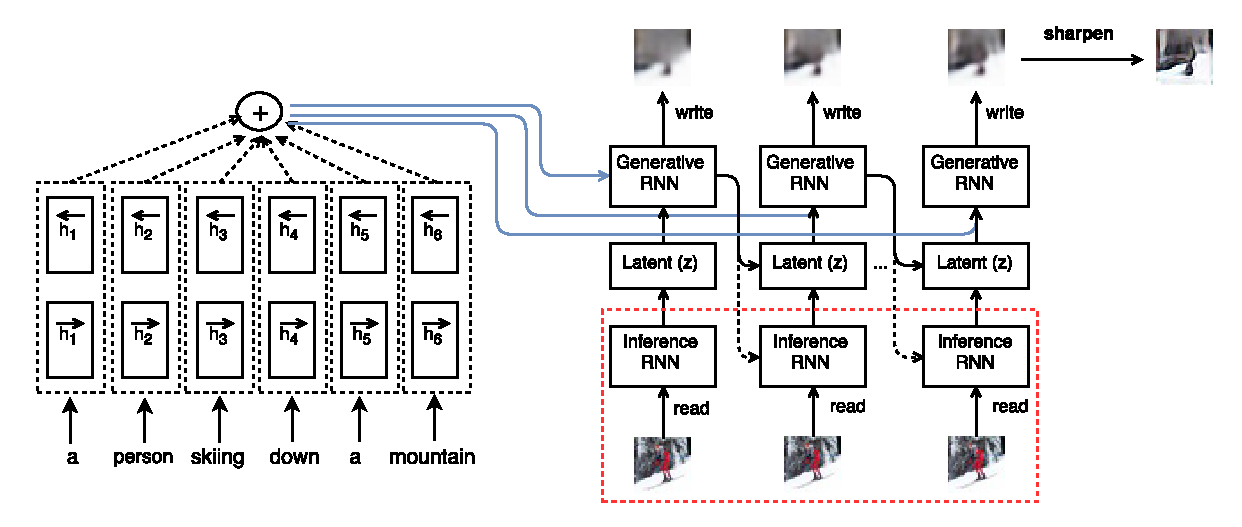
\includegraphics[width=0.8\textwidth]{figures/alignDraw-cropped.pdf}\quad
%
\end{center}
\vspace{-0.2in}
\caption{The image of the proposed model}
\label{fig:figmodel}
\vspace{-1cm}
\end{figure}
\vspace{-0.1in}

Let $\icaption$ be the input caption, consisting of $N$ words $y_{1}, y_{2}, ..., y_{N}$, and $\oimage$ be the output image. Our proposed model 
defines a generative process of images conditioned the caption. In particular, captions are represented as a sequence of consecutive words and images are represented as a sequence of patches drawn on canvas over time $t=1,...,T$. Our model can be viewed as utilizing the  sequence-to-sequence framework \citep{ilya_mt}, \citep{cho_mt}, \citep{nitish_video}.  

\subsection{Language Representation: the Bidirectional Attention RNN}
\label{sec:lang}
We obtain the caption sentence representation by first transforming each word $y_{1},...,y_{N}$ to a vector representation using the Bidirectional RNN\cite{}. In a Bidrectional RNN, the two LSTM process the input sequence from both forward and backward directions. The two LSTMs produces the hidden states sequences $[\overrightarrow{h}^{lang}_{1}, \overrightarrow{h}^{lang}_{2}, ..., \overrightarrow{h}^{lang}_{N}]$ and $[\overleftarrow{h}^{lang}_{1}, \overleftarrow{h}^{lang}_{2}, ..., \overleftarrow{h}^{lang}_{N}]$ respectively. Then these hidden states are concatenated together into the final sentence representation $\hlangall = [\hlang_{1}, \hlang_{2}, ..., \hlang_{N}]$, where $\hlang_{n} = [\overrightarrow{h}^{lang}_{n}, \overleftarrow{h}^{lang}_{n}], 1\leq n\leq N$.


\subsection{Image Modelling: the Conditional alginDRAW Network}
\comm{
The DRAW network \cite{gregor_draw} is a sequential probabilistic model generating images by accumulating the output at each iterative step. While the original DRAW network assumes the latent variables are independent, it has shown in \citep{bachman_sdm} the model performance is improved by including the dependencies of latent variables. 
}
To generate images conditioned on the caption information, we extended the DRAW network\citep{gregor_draw} to include caption representation $\hlangall$ at each step, shown in Figure (\ref{fig:figmodel}). The conditional DRAW network is a stochastic recurrent neural network that consists of a set of latent variables $\Lat_t$ at each time step. Unlike the original DRAW network where latent variables are independent unit Gaussian $\mathcal{N}(0, I)$, the latent variables in the alignDRAW model have their mean and variance depends on the previous recurrent hidden states $\hdec_{t-1}$ as in \cite{bachman_sdm}. Formally, the image is generated by iteratively computing the following equations for $t=1,...,T$
\begin{align}
\vspace{-0.1in}
\label{eq:x_hat}
\lat_t &\sim \prior(\Lat_t|\Lat_{1:t-1}) = \mathcal{N}(\mu_{t}(\hdec_{t-1}), \sigma_{t}(\hdec_{t-1}))\\
\hdec_t &= \decoder(\hdec_{t-1}, z_t, s_{t-1})\\
s_{t} &= align(\hdec_{t-1}, \hlangall) \\
\label{eq:write}
\canv_t &= \canv_{t-1} + \writeop(\hdec_t)
\end{align}
where $\readop$ and $\writeop$ are the same attention operators as in \citep{gregor_draw}.
The $align$ function is used to compute the alignment between the input caption and intermediate image generative steps as in \cite{bahdanau_mt}. Given the caption representation from the language model, $\hlangall = [\hlang_{1}, \hlang_{2}, ..., \hlang_{N}]$, the $align$ operator computes the final sentence representation $s_t$ through a weighted sum using alignment probabilities $\alpha_{1...N}$:
\begin{align}
\vspace{-0.1in}
s_t=align(\hdec_{t-1}, \hlangall) = \alpha_{1}\hlang_{1} + \alpha_{2}\hlang_{2} + ... + \alpha_{N}\hlang_{N}.
\end{align}
The corresponding alignment probabilities $\alpha_{1...N}$ at each step are obtained using the caption representation $\hlang$ and the hidden state of the generative model $\hdec_{t}$, as in \citep{bahdanau_mt}
\comm{
\begin{align}
e_{tj} &= v^{T}tanh(U\hlang_{j} + W\hdec_{t} + b)\\
\alpha_{j} &= \frac{exp(e_{tj})}{\sum_{j=1}^{N}exp(e_{tj})}.
\end{align}
}
\comm{
Here $\hlang_{0}$ is initialized to the learned bias.
Setting $\alpha_{1...N}$ to $\frac{1}{N}$ turns the encoder into the vanilla model introduced in \citep{cho_mt} without the attention. 
}
\subsection{Learning}

Our conditional alignDRAW model is trained to maximize the variational lower bound on the log-likelihood, $\log \sum_{\Lat_{1:T}} \prior(\Lat_{1:T})p(\oimage\given\icaption, \Lat_{1:T})$. The posterior inference is approximated by an inference RNN $\post(\Lat_{1:T}\given\icaption,\oimage)$ shown in red dash box in Figure (\ref{fig:figmodel}).   
Overall, the variational objective $\loss$ is defined with the model parameters vector $\theta_\theta$ as follows:
\begin{align}
\vspace{-0.1in}
\loss_\theta =  &\expectation_{\post(\Lat_{1:t}\given\icaption,\oimage)}\left[ - \log p(\oimage\given\icaption,\Lat_{1:T}) + \sum_{t=2}^T\kldiv\left(\post(\Lat_t\given\Lat_{1:t-1},\icaption,\oimage)\klBars\prior(\Lat_t\given\Lat_{1:t-1},\icaption)\right) \right] \nonumber \\& + \kldiv\left(\post(\Lat_1\given\oimage)\klBars\prior(\Lat_1\given\icaption)\right).
\end{align}




\comm{
is learned by the modified version of Stochastic Gradient Variation Bayes (SGVB) algorithm introduced by \cite{kingma_vae}. The model is trained to maximize the lower bound of marginal likelihood $\loss$ of the correct image $x$ given the input caption $y$. The $\loss$ is decomposed into the latent loss $\lloss$ and the reconstruction loss $\rloss$. 

The reconstruction loss $\rloss$ equals to $\frac{1}{L}\sum_{l=1}^{L}(log\,p(x_{t}|y,z)$ where $L$ is the number of samples used during training, which was set to $1$ in our experiments.

The latent loss $\lloss$ is a negative sum of Kullback--Leibler divergence terms between distribution $\post(\Lat_t|\henc_t)$ and some prior distribution ${\prior(\Lat_t)}$ over time $t=1,...,T$, which can be seen as a regularization term. Since the patches drawn on canvas over time are not independent of each other, naturally the sufficient statistics of the prior distribution at time $t$ should be dependent on the sufficient statistics of the prior distribution at time $t-1$. Therefore, instead of setting $\prior(\Lat_1), ..., \prior(\Lat_T)$ to be independent unit gaussian distributions, the mean and variance of $\prior(\Lat_t)$ depends on the $\hdec_{t-1}$, which forms a Markov chain $\prior(\Lat_1), \prior(\Lat_2\given\Lat_1), ..., \prior(\Lat_T\given\Lat_{T-1})$ as in \citep{bachman_sdm}, where 
\begin{align}
\mu_{t}^{prior} &= tanh(W_{\mu}\hdec_{t-1})\\
\sigma_{t}^{prior} &= exp(tanh(W_{\sigma}\hdec_{t-1})) 
\end{align}
}
\comm{
The expectation can be approximate by $\numSamples$ Monte Carlo samples $\LatSample_{1:T}$ from $\post(\Lat_{1:T}\given\icaption, \oimage)$:
\begin{align}
\loss \approx  &\frac{1}{\numSamples}\sum_{\sampleIdx=1}^\numSamples\left[ - \log p(\oimage\given\icaption,\LatSample^\sampleIdx_{1:T}) + \sum_{t=2}^T\kldiv\left(\post(\Lat_t\given\LatSample^\sampleIdx_{t-1},\icaption,\oimage)\klBars\prior(\Lat_t\given\LatSample^\sampleIdx_{t-1},\icaption)\right) \right] \nonumber \\& + \kldiv\left(\post(\Lat_1\given\icaption,\oimage)\klBars\prior(\Lat_1\given\icaption)\right).
\end{align}
\comm{
\begin{align}
\loss &= -\sum_{t=1}^{T}D_{KL}(\post(\Lat_t|\henc_t,s_{t-1})\,||\,\prior(\Lat_t)) + \frac{1}{L}\sum_{l=1}^{L}log\,p(x_{t}|y,z)\\
&=
\frac{1}{2}\sum_{t=1}^{T}(1 - 2\,log\,\sigma_{t}^{prior} + 2\,log\,\sigma_{t} - \frac{exp(2\,log\,\sigma_{t}) + (\mu_{t} - \mu_{t}^{prior})^{2}}{exp(2\,log\,\sigma_{t}^{prior})}) + \frac{1}{L}\sum_{l=1}^{L}log\,p(x_{t}|y,z)
\end{align}
}
}
\subsection{Generating Images from Captions}

At the test time, images are generated by ancestral sampling the latent variables from the prior $\prior(\Lat_{1:T})$. Due to the blurriness of samples generated by the alignDRAW model, the blurry samples are fed to an additional post processing step. The generator of an adversarial network, trained independently on the residuals of a Laplacian pyramid, is used to sharpen the generated images from alignDRAW. The adversarial network is conditioned on the input caption using skip-thought vector\cite{skip-thought} and is trained similar to \citep{denton_lapgan}.    
Instead of sampling from its prior, we fix the adversarial generator to be the mean of the original uniform distribution. This post-processing step is a deterministic mapping which enable us to calculate the lower bound on the new log-likelihood defined at the output of the adversarial generator. Interestingly, we also found the deterministic procoess generate samples with much less noise than if we had sampled from the uniform distribution.

\comm{. The reconstruction loss becomes the loss between sharpened image and correct image, whereas the latent loss stays the same. We also noticed that inputting the mean of the uniform distribution into the edge generator network allowed us to generate samples with much less noise than if we had sampled from the uniform distribution.  }

\section{Experiments}
% \subsection{MNIST With Captions}
% As a toy experiment, we have trained our model on the two digit MNIST dataset with captions constructed on the fly. Two random digits were either placed horizontally or vertically, so that they don't overlap, on the black $60 \times 60$ background. The caption indicated the way digits were placed in the image and had the following template: \textit{the digit (1) is (2) the (3) of the digit (4) \textless eos\textgreater}. (1) and (4) were the digit numbers, (2) was either on or at, (3) was one of the adjectives top, bottom, left or right. For example, the generated images corresponding to the caption \textit{the digit seven is at the bottom of the digit five \textless eos\textgreater} as well as other captions are shown on~\ref{fig:fig1}. While most of the generative models were trained on the version of binarized MNIST dataset \citep{russ_binarizedmnist}, our model was trained directly on pixel intensities with binary cross entropy cost function.

% \begin{figure}[t]
% \label{fig1}
% \captionsetup{labelformat=empty}
% \minipage{0.1\textwidth}
%   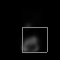
\includegraphics[width=\linewidth]{figures/5-7-4.png}
%   \caption{\textit{is digit 5}}
% \endminipage\hfill
% \minipage{0.1\textwidth}
%   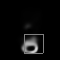
\includegraphics[width=\linewidth]{figures/5-7-6.png}
%   \caption{\textit{is digit 5}}
% \endminipage\hfill
% \minipage{0.1\textwidth}
%   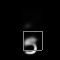
\includegraphics[width=\linewidth]{figures/5-7-9.png}
%   \caption{\textit{is digit 5}}
% \endminipage\hfill
% \minipage{0.1\textwidth}
%   
\includegraphics[width=\linewidth]{figures/5-7-13.png}
%   \caption{\textit{is digit 5}}
% \endminipage\hfill
% \minipage{0.1\textwidth}
%   
\includegraphics[width=\linewidth]{figures/5-7-17.png}
%   \caption{\mbox{\textit{eos 7 digit}}}
% \endminipage\hfill
% \minipage{0.1\textwidth}
%   
\includegraphics[width=\linewidth]{figures/5-7-22.png}
%   \caption{\mbox{\textit{eos 7 digit}}}
% \endminipage\hfill
% \minipage{0.1\textwidth}
%   
\includegraphics[width=\linewidth]{figures/5-7-26.png}
%   \caption{\mbox{\textit{eos 7 digit}}}
% \endminipage\hfill
% \minipage{0.1\textwidth}
%   
\includegraphics[width=\linewidth]{figures/5-7-27.png}
%   \caption{\mbox{\textit{eos 7 digit}}}
% \endminipage\hfill

% \minipage{0.1\textwidth}
%   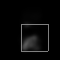
\includegraphics[width=\linewidth]{figures/9-2-4.png}
%   \caption{\mbox{\textit{eos digit 2}}}
% \endminipage\hfill
% \minipage{0.1\textwidth}
%   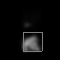
\includegraphics[width=\linewidth]{figures/9-2-6.png}
%   \caption{\mbox{\textit{eos digit 2}}}
% \endminipage\hfill
% \minipage{0.1\textwidth}
%   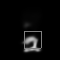
\includegraphics[width=\linewidth]{figures/9-2-9.png}
%   \caption{\mbox{\textit{eos digit 2}}}
% \endminipage\hfill
% \minipage{0.1\textwidth}
%   
\includegraphics[width=\linewidth]{figures/9-2-13.png}
%   \caption{\mbox{\textit{eos digit 2}}}
% \endminipage\hfill
% \minipage{0.1\textwidth}
%   
\includegraphics[width=\linewidth]{figures/9-2-17.png}
%   \caption{\mbox{\textit{of top digit}}}
% \endminipage\hfill
% \minipage{0.1\textwidth}
%   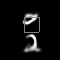
\includegraphics[width=\linewidth]{figures/9-2-22.png}
%   \caption{\mbox{\textit{of top digit}}}
% \endminipage\hfill
% \minipage{0.1\textwidth}
%   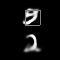
\includegraphics[width=\linewidth]{figures/9-2-26.png}
%   \caption{\mbox{\textit{of top digit}}}
% \endminipage\hfill
% \minipage{0.1\textwidth}
%   
\includegraphics[width=\linewidth]{figures/9-2-27.png}
%   \caption{\mbox{\textit{of top digit}}}
% \endminipage\hfill

% \minipage{0.1\textwidth}
%   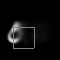
\includegraphics[width=\linewidth]{figures/1-0-4.png}
%   \caption{\mbox{\textit{eos 0 of}}}
% \endminipage\hfill
% \minipage{0.1\textwidth}
%   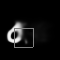
\includegraphics[width=\linewidth]{figures/1-0-6.png}
%   \caption{\mbox{\textit{eos digit 0}}}
% \endminipage\hfill
% \minipage{0.1\textwidth}
%   
\includegraphics[width=\linewidth]{figures/1-0-9.png}
%   \caption{\mbox{\textit{eos digit 0}}}
% \endminipage\hfill
% \minipage{0.1\textwidth}
%   
\includegraphics[width=\linewidth]{figures/1-0-12.png}
%   \caption{\mbox{\textit{eos 0 of}}}
% \endminipage\hfill
% \minipage{0.1\textwidth}
%   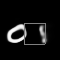
\includegraphics[width=\linewidth]{figures/1-0-17.png}
%   \caption{\mbox{\textit{1 digit the}}}
% \endminipage\hfill
% \minipage{0.1\textwidth}
%   
\includegraphics[width=\linewidth]{figures/1-0-22.png}
%   \caption{\mbox{\textit{1 digit the}}}
% \endminipage\hfill
% \minipage{0.1\textwidth}
%   
\includegraphics[width=\linewidth]{figures/1-0-25.png}
%   \caption{\mbox{\textit{1 digit on}}}
% \endminipage\hfill
% \minipage{0.1\textwidth}
%   
\includegraphics[width=\linewidth]{figures/1-0-28.png}
%   \caption{\mbox{\textit{digit the eos}}}
% \endminipage\hfill

% \minipage{0.1\textwidth}
%   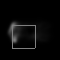
\includegraphics[width=\linewidth]{figures/4-8-4.png}
%   \caption{\textit{left 8 4}}
% \endminipage\hfill
% \minipage{0.1\textwidth}
%   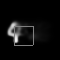
\includegraphics[width=\linewidth]{figures/4-8-6.png}
%   \caption{\textit{left 8 4}}
% \endminipage\hfill
% \minipage{0.1\textwidth}
%   
\includegraphics[width=\linewidth]{figures/4-8-9.png}
%   \caption{\mbox{\textit{left digit 4}}}
% \endminipage\hfill
% \minipage{0.1\textwidth}
%   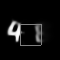
\includegraphics[width=\linewidth]{figures/4-8-14.png}
%   \caption{\mbox{\textit{eos 8 digit}}}
% \endminipage\hfill
% \minipage{0.1\textwidth}
%   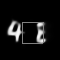
\includegraphics[width=\linewidth]{figures/4-8-18.png}
%   \caption{\mbox{\textit{eos 8 digit}}}
% \endminipage\hfill
% \minipage{0.1\textwidth}
%   
\includegraphics[width=\linewidth]{figures/4-8-22.png}
%   \caption{\mbox{\textit{8 digit the}}}
% \endminipage\hfill
% \minipage{0.1\textwidth}
%   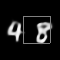
\includegraphics[width=\linewidth]{figures/4-8-25.png}
%   \caption{\mbox{\textit{8 digit digit}}}
% \endminipage\hfill
% \minipage{0.1\textwidth}
%   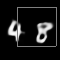
\includegraphics[width=\linewidth]{figures/4-8-28.png}
%   \caption{\mbox{\textit{digit digit the}}}
% \endminipage\hfill

% \captionsetup{labelformat=empty}
% \caption{Figure 1: Four examples show the generated images unfolded over several timesteps as well as the top three words the model attends to while generating images.}
% \end{figure}

\subsection{COCO}

Microsoft COCO \citep{mscoco} is a very large dataset of roughly 83k images, each annotated with 5 captions. The rich collection of images with a wide variety of styles, backgrounds and objects makes the task of learning a good generative model conditioned on a caption very challenging. For consistency with related work on caption generation, we disregard four of the five captions when training our model.
%Since some of the images have more than five captions attached to them, 

In the following subsections, we analyze both the qualitative and quantitative aspects of our model as well as compare its performance with that of other, related generative models.

\subsubsection{Analysis of Generated Images}
The main goal of this work is to learn a model that can understand the semantic meaning expressed in the textual descriptions of images, such as the properties of objects, the relationships between them, etc. and then use that knowledge to generate relevant images. To verify that, we wrote a set of captions inspired by the COCO dataset and changed some words in the captions to see whether the model made the relevant changes in the generated samples.

First, we wanted to see whether the model understood one of the most basic properties of any object, the color. In Figure~\ref{fig:genimages1}, we generated images of school buses with four different colors: yellow, red, green and blue. Although, there are images of buses with different colors in the training set, all mentioned school buses are specifically colored yellow. Despite that, the model managed to generate images of an object that is visually reminiscent of a school bus that is painted with the specified color.

\begin{figure}[!h]
\captionsetup[subfigure]{labelformat=empty}
\begin{center}
\subfloat[A \underline{yellow} school bus parked in a parking lot.
]{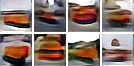
\includegraphics[width=0.23\textwidth]{figures/new/a-yellow-school-bus-parked-in-a-parking-lot-sharp.png}}\quad
%
\subfloat[A \underline{red} school bus parked in a parking lot.
]{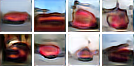
\includegraphics[width=0.23\textwidth]{figures/new/a-red-school-bus-parked-in-a-parking-lot-sharp.png}}\quad
%
\subfloat[A \underline{green} school bus parked in a parking lot.
]{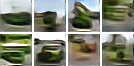
\includegraphics[width=0.23\textwidth]{figures/new/a-green-school-bus-parked-in-a-parking-lot-sharp.png}}\quad
%
\subfloat[A \underline{blue} school bus parked in a parking lot.
]{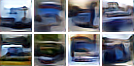
\includegraphics[width=0.23\textwidth]{figures/new/a-blue-school-bus-parked-in-a-parking-lot-sharp.png}}\quad
%
\end{center}
\caption{Examples of changing the color while keeping the caption fixed.}
\label{fig:genimages1}
\vspace{-0.3cm}
\end{figure}

Apart from changing the colors of objects, we were curious whether changing the background of the scene described in a caption would result in the appropriate changes in the generated samples. The task of changing the background of an image is somewhat harder than just changing the color of an object because the model will have to make alterations over a wider visual area. Nevertheless, as shown in Figure~\ref{fig:genimages2} changing the skies from blue to rainy in a caption as well as changing the grass type from dry to green in another caption resulted in the appropriate changes in the generated image. The nearest images from the training set also indicate that the model was not simply copying the patterns it observed during the learning phase.

\begin{figure}[!h]
\captionsetup[subfigure]{labelformat=empty}
\begin{center}
\subfloat[]{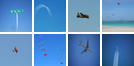
\includegraphics[width=0.23\textwidth]{figures/new/a-very-large-commercial-plane-flying-in-blue-skies-closest.png}}\quad
%
\subfloat[]{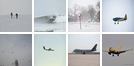
\includegraphics[width=0.23\textwidth]{figures/new/a-very-large-commercial-plane-flying-in-rainy-skies-closest.png}}\quad
%
\subfloat[]{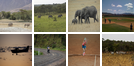
\includegraphics[width=0.23\textwidth]{figures/new/a-herd-of-elephants-walking-across-a-dry-grass-field-closest.png}}\quad
%
\subfloat[]{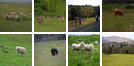
\includegraphics[width=0.23\textwidth]{figures/new/a-herd-of-elephants-walking-across-a-green-grass-field-closest.png}}\\
\vspace{-0.45cm}
%
\subfloat[A very large commercial plane flying in \underline{blue} skies.
]{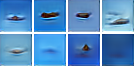
\includegraphics[width=0.23\textwidth]{figures/new/a-very-large-commercial-plane-flying-in-blue-skies-sharp.png}}\quad
%
\subfloat[A very large commercial plane flying in \underline{rainy} skies.
]{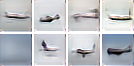
\includegraphics[width=0.23\textwidth]{figures/new/a-very-large-commercial-plane-flying-in-rainy-skies-sharp.png}}\quad
%
\subfloat[A herd of elephants walking across a \underline{dry} grass field.
]{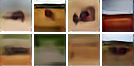
\includegraphics[width=0.23\textwidth]{figures/new/a-herd-of-elephants-walking-across-a-dry-grass-field-sharp.png}}\quad
%
\subfloat[A herd of elephants walking across a \underline{green} grass field.
]{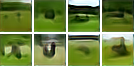
\includegraphics[width=0.23\textwidth]{figures/new/a-herd-of-elephants-walking-across-a-green-grass-field-sharp.png}}\quad
%
\end{center}
\caption{Bottom: Examples of changing the background while keeping the caption fixed. Top: The respective nearest training images based on pixel-wise L2 distance.}
\label{fig:genimages2}
\vspace{-0.3cm}
\end{figure}

Despite an infinite number of ways of changing colors and backgrounds in descriptions, in general we found that the model made appropriate changes as long as some similar pattern was present in the training set. However, the model struggled when the visual difference between objects was very small, such as when the objects have the same general shape and color. In Figure~\ref{fig:genimages3}, we demonstrate that when we swap two objects that are both visually similar, for example cats and dogs, it is difficult to discriminate solely from the generated samples whether it is an image of a cat or dog, even though we might notice an animal-like shape. This highlights a limitation of the model in that it has difficulty modelling the fine-grained details of objects. 
 
\begin{figure}[!h]
\captionsetup[subfigure]{labelformat=empty}
\begin{center}
\subfloat[\underline{The decadent chocolate} \underline{desert} is on the table.
]{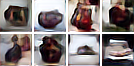
\includegraphics[width=0.23\textwidth]{figures/new/the-decadent-chocolate-dessert-is-on-the-table-sharp.png}}\quad
%
\subfloat[\underline{A bowl of bananas} is on the table.
]{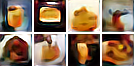
\includegraphics[width=0.23\textwidth]{figures/new/a-bowl-of-bananas-is-on-the-table-sharp.png}}\quad
%
\subfloat[A vintage photo of a \underline{cat}.
]{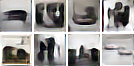
\includegraphics[width=0.23\textwidth]{figures/new/a-vintage-photo-of-a-cat-sharp.png}}\quad
%
\subfloat[A vintage photo of a \underline{dog}.
]{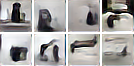
\includegraphics[width=0.23\textwidth]{figures/new/a-vintage-photo-of-a-dog-sharp.png}}\quad
%
\end{center}
\caption{Examples of changing the object while keeping the caption fixed.}
\label{fig:genimages3}
\vspace{-0.3cm}
\end{figure}

\subsubsection{Analysis of Attention}

After flipping sets of words in the captions, we were curious to see which words the model attended to when generating images. It turned out that during the generation step, the model mostly focused on the specific words (or their neighbors) that carried the main semantic meaning expressed in the sentences. The attention values in sentences helped us interpret the reasons why the model made the changes it did when we flipped certain words. For example, in Figure~\ref{fig:attentimages1} we can see that when we flipped the word ``desert'' to ``forest'', the attention over words in the sentence did not change drastically. This suggests that, in their respective sentences, the model looked at ``desert'' and ``forest'' with relatively equal probability, and thus made the correct changes. In contrast, when we swap words ``beach'' and ``sun'', we can see a drastic change between sentences in the probability distribution over words. By noting that the model completely ignores the word ``sun'' in the second sentence, we can therefore gain a more thorough understanding of why we see no visual differences between the images generated by each caption.

We also tried to analyze the way the model generated images. Unfortunately, we found that there was no connection between the patches drawn on canvas and the most attended words at particular timesteps.

\begin{figure}[!h]
\captionsetup[subfigure]{labelformat=empty}
\begin{center}
\subfloat[\hlcthree{A} rider \hlcone{on} a blue \hlcone{motorcycle} in the \underline{\hlctwo{desert}}.
]{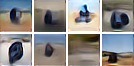
\includegraphics[width=0.23\textwidth]{figures/new/a-rider-on-a-blue-motorcycle-in-the-desert-sharp.png}}\quad
%
\subfloat[\hlcthree{A} rider \hlcone{on} a blue \hlcone{motorcycle} in the \underline{\hlctwo{forest}}.
]{\includegraphics[width=0.23\textwidth]{figures/new/a-rider-on-a-blue-motorcycle-in-the-forest-sharp.png}}\quad
%
\subfloat[\hlctwo{A} \hlcone{surfer}, a woman, and a child walk on the \underline{\hlctwo{beach}}.
]{\includegraphics[width=0.23\textwidth]{figures/new/a-surfer-,-a-woman-,-and-a-child-walk-on-the-beach-sharp.png}}\quad
%
\subfloat[\hlcthree{A} \hlcone{surfer}, a woman, and a child walk on the \underline{\hlczero{sun}}.
]{\includegraphics[width=0.23\textwidth]{figures/new/a-surfer-,-a-woman-,-and-a-child-walk-on-the-sun-sharp.png}}\quad
%
\end{center}
\caption{Examples of most attended words while changing the background in the caption.}
\label{fig:attentimages1}
\vspace{-0.3cm}
\end{figure} 

\subsubsection{Comparison With Other Models}
Quantitatively evaluating generative models remains a challenging task in of itself as each method of evaluation suffer from its own specific drawbacks. Compared to reporting classification accuracies in discriminative models, the measures defining generative models are intractable most of the times and might not correctly define the real quality of the model. To get a better comparison between performances of different generative models, we report results on two different metrics as well as a qualitative comparison of different generative models.

\begin{figure}[!t]
\captionsetup[subfigure]{labelformat=empty}
\begin{center}
\subfloat[Align DRAW]{\includegraphics[width=0.23\textwidth]{figures/new/a-group-of-people-walk-on-a-beach-with-surf-boards-sharp.png}}\quad
%
\subfloat[LAPGAN]{\includegraphics[width=0.23\textwidth]{figures/a-group-of-people-walk-on-a-beach-with-surf-boards-lapgan.png}}\quad
%
\subfloat[Conv. VAE]{\includegraphics[width=0.23\textwidth]{figures/a-group-of-people-walk-on-a-beach-with-surf-boards-convdeconvvae.png}}\quad
%
\subfloat[Fully-conn. VAE]{\includegraphics[width=0.23\textwidth]{figures/a-group-of-people-walk-on-a-beach-with-surf-boards-fcvae.png}}\quad
%
\end{center}
\caption{Four different models displaying results from sampling caption \textit{A group of people walk on a beach with surf boards.}}
\label{fig:diffmodels}
\vspace{-0.2cm}
\end{figure}

In Figure~\ref{fig:diffmodels}, we generated several samples from the prior of each of the current state-of-the-art generative models, conditioned on the caption ``A group of people walk on a beach with surf boards". While all of the samples look sharp, the images generated by LAPGAN look more noisy and it is harder to make out definite objects, 
%don't have a clear structure in them
whereas the images generated by variational models trained with L2 cost function have a watercolor effect on the images.

As for the quantitative comparison of different models, we first compare the performances of the model trained with variational methods. We rank the images in test set conditioned on the captions based on the variational lower bound of likelihood and then report the Precision-Recall metric to evaluate the quality of the generative model. Unsurprisingly, the quality of image retrieval using generative models is worse than that of discriminative models that were specifically built for retrieval. To deal with the large computational complexity involved in looping through each test image, we create a shortlist of one hundred images including the correct one, based on the images having the closest distance in the convolutional feature-space of a VGG-like model trained on the CIFAR dataset. Since there are ``easy'' images for which the model assigns high likelihood independent of the query caption, we look at the ratio of likelihood of image conditioned on the sentence to likelihood of image conditioned on the mean sentence representation in the training set. We found that the reconstruction error $\rloss$ increased for sharpened images, and that sharpening considerably hurt the retrieval results. Since sharpening changes the statistics of images, computing reconstruction error for each pixel is not necessarily a good metric.

Instead of calculating error per pixel, we turn to a smarter metric, the Structural Similarity Index (SSI), which incorporates luminance and contrast masking into the error calculation. Due to strong inter-dependencies of closer pixels, the metric is calculated on small windows of the image. To calculate SSI, we sampled fifty images from the prior of each generative model for every caption in the test set.

\begin{table}[!b]
\begin{center}
\begin{tabulary}{\linewidth}{c || c c c c c || c}
\hline
\multicolumn{7}{c}{\textbf{COCO (before sharpening)}} \\
\hline
& \multicolumn{5}{c||}{Image Search} & Image Similarity \\
%\cline{2-6}
\textbf{Model} & \textbf{R@1} & \textbf{R@5} & \textbf{R@10} & \textbf{R@50} & \textbf{Med r} & \textbf{SSI} \\
\hline
\hline
LAPGAN & - & - & - & - & - & 0.08 \\ % - & - & - & - & - & 0.08
\hline
Fully-conn. VAE (L2 cost) & 1.0 & 5.6 & 10.4 & 51.1 & 51 & 0.156 \\ % 0.688 & 4.58 & 8.74 & 46.832 & 54 & -1
Conv. VAE (L2 cost) & 1.0 & 5.9 & 10.9 & 50.8 & 50 & \textbf{0.164} \\ % 0.672 & 4.448 & 8.476 & 46.596 & 54 & 0.131
Skipthought DRAW & 2.0 & 11.2 & 18.9 & 63.3 & 36 & 0.157 \\ % 0.988 & 6.18 & 11.48 & 52.512 & 48 & 0.118
Noalign DRAW & 2.8 & \textbf{14.1} & \textbf{23.1} & 68.0 & \textbf{31} & 0.155 \\ % 1.0 & 6.124 & 11.18 & 52.112 & 48 & 0.114
Align DRAW & \textbf{3.0} & 14.0 & 22.9 & \textbf{68.5} & \textbf{31} & 0.156 \\ % 0.924 & 6.216 & 11.184 & 52.492 & 48 & 0.115
\end{tabulary}
\end{center}
\end{table}

{\footnotesize
\bibliography{ram-paper}}

\end{document}
